% IMPORTANT: PLEASE USE XeLaTeX FOR TYPESETTING
\documentclass{sintefbeamer}
\usepackage{xeCJK}
\usepackage{amsthm}
\setbeamertemplate{theorems}[numbered]
\makeatletter
\setbeamertemplate{footline}
{
  \leavevmode%
  \hbox{%
  \begin{beamercolorbox}[wd=.7\paperwidth,ht=2.25ex,dp=1ex,center]{title in head/foot}%
    \usebeamerfont{title in head/foot} {基于数据生成的类别均衡联邦学习}
  \end{beamercolorbox}%
  \begin{beamercolorbox}[wd=.3\paperwidth,ht=2.25ex,dp=1ex,right]{date in head/foot}%
    \usebeamerfont{date in head/foot}\insertshortdate{}\hspace*{2em}
    \insertframenumber{} / \inserttotalframenumber\hspace*{2ex} 
  \end{beamercolorbox}}%
  \vskip0pt%
}

%\newtheorem{theorem}{Theorem} % to number according to section
\theoremstyle{definition}

\makeatother

% meta-data
\title{\huge 基于数据生成的类别均衡联邦学习}
\subtitle{汇报人:黄其涵 \qquad 导师:章静 教授 \qquad }
\author{计算机学报, 2023}
\date{\today}
\titlebackground{images/bg4}

% document body
\begin{document}

\maketitle


\section{研究背景}

\begin{frame}{1.1 联邦学习}
\begin{itemize}
\item 联邦学习是一种分布式机器学习方法,其利用一个中央服务器(也称为服务器端)协调各终端设备(也称为客户端),协同训练一个各客户端共享的全局模型。

\item 与传统中心化训练方法不同,\textbf{联邦学习不需要各设备发送自身隐私数据至数据中心,因此有利于保护数据隐私。}具体而言,联邦学习在客户端和服务器端之间通过多轮通信迭代优化模型。
\item 每轮通信包含两个阶段:
\begin{itemize}
\item[(1)]各客户端从服务器端下载全局模型,并在本地数据上进行训练以获得本地模型;
\item[(2)]服务器端接收并聚合各客户端的本地模型参数以获得性能更优的全局模型.然而,现有联邦学习机制尚面临两大不足。
\end{itemize}
\end{itemize}



\end{frame}

\begin{frame}{1.2 现有问题}
\begin{columns}
\begin{column}{0.45\textwidth}
\begin{figure}[ht]
\centering
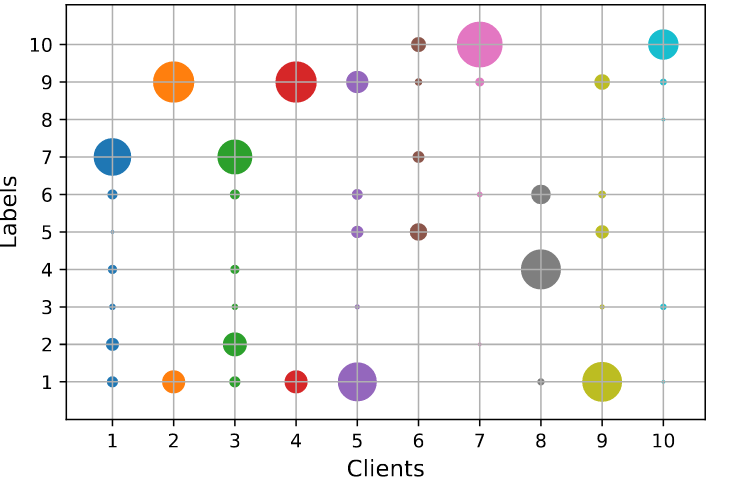
\includegraphics[width=1\textwidth]{images/img_unbalance}
\end{figure}
\end{column}
\begin{column}{0.65\textwidth}
\begin{itemize}
\item \textbf{类别不均衡。}全局模型需考虑多个客户端的数据,但各客户端往往仅包含部分类别数据且类别间数据量严重不均衡,使得全局模型难以训练。所训练的本地模型容易过拟合本地数据而在全局数据上往往取得较差性能。更重要的是,这些性能较差的本地模型严重影响全局模型的训练,导致难以构建高性能全局模型。
\item \textbf{数据分布差异。}由于各客户端的功能和用户使用习惯不同,不同客户端往往产生不同类别的数据,导致各客户端数据之间的类别分布差异较大。
\end{itemize}
\end{column}
\end{columns}
\end{frame}


\begin{frame}{1.3 主要贡献}
\begin{itemize}
\item \textbf{本文提出类别分布均衡器来均衡客户终端的类别分布。}其中,类别分布均衡器由类别均衡采集样器和数据生成器组成。类别均衡采样器对客户端数据量不足的类别以较高概率进行采样,数据生成器则根据所采样的类别生成相应的虚拟数据;
\item \textbf{基于类别分布均衡器,本文提出一种新颖的类别均衡联邦学习方法(CBFL)。}CBFL在客户端构造类别均衡的数据集进行训练,从而提高各本地模型的性能并减少各本地模型之间的差异性,进而构建高性能全局模型;
\item \textbf{本文在四个标准数据集上进行了大量实验,证明了所提出CBFL的有效性.}与最新方法相比,CBFL在多种深度神经网络(如ResNet20和MobileNetV2)取得更优越的性能.尤其在客户端上类别分布高度不均衡且客户端之间类别分布差异巨大的情况下,CBFL比现有方法具有更大的优势.
\end{itemize}
\end{frame}

\section{问题定义}

\begin{frame}{2 优化目标}

\begin{columns}
\begin{column}{0.4\textwidth}
\begin{figure}[ht]
\centering
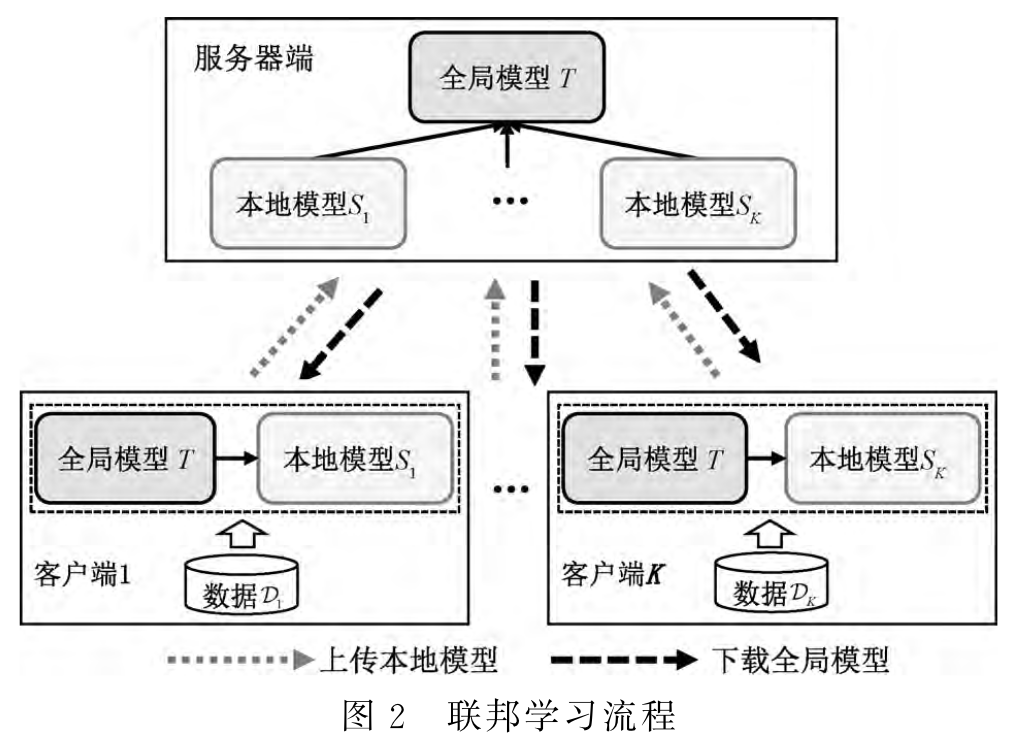
\includegraphics[width=1\textwidth]{images/img_fl}
\end{figure}
\end{column}
\begin{column}{0.6\textwidth}
为解决上述难题, 本文提出在客户端构造类别均衡的数据集进行训练的策略。 令 $\mathcal{D}$ 表示所构造的类别 均衡数 据集, $M$ 表示全局数据的类别数,则 $\mathcal{D}=\left\{(x, y) \mid P(y=i)=\frac{1}{M}, \quad i \in\{0,1, \ldots, M-1\}\right.$.
$p(\mathcal{D})$ 表示数据集 $\mathcal{D}$ 所代表的经验分布. 因此, 本文 旨在解决如下优化问题:
$$
\min _{\boldsymbol{W}_T} \mathbb{E}_k\left[\mathbb{E}_{x_k \sim p(\mathcal{D})}\left[\mathcal{L}\left(x_k ; \boldsymbol{W}_T\right)\right]\right]
$$
与仅仅利用客户端本地数据进行训练的方式相比,基于类别均衡的数据集进行训练使得各客户端本地模型之间的差异大大减少。
\end{column}
\end{columns}


\end{frame}

\section{研究方法}

\begin{frame}{3.1 CBFL方案框架}
\centering
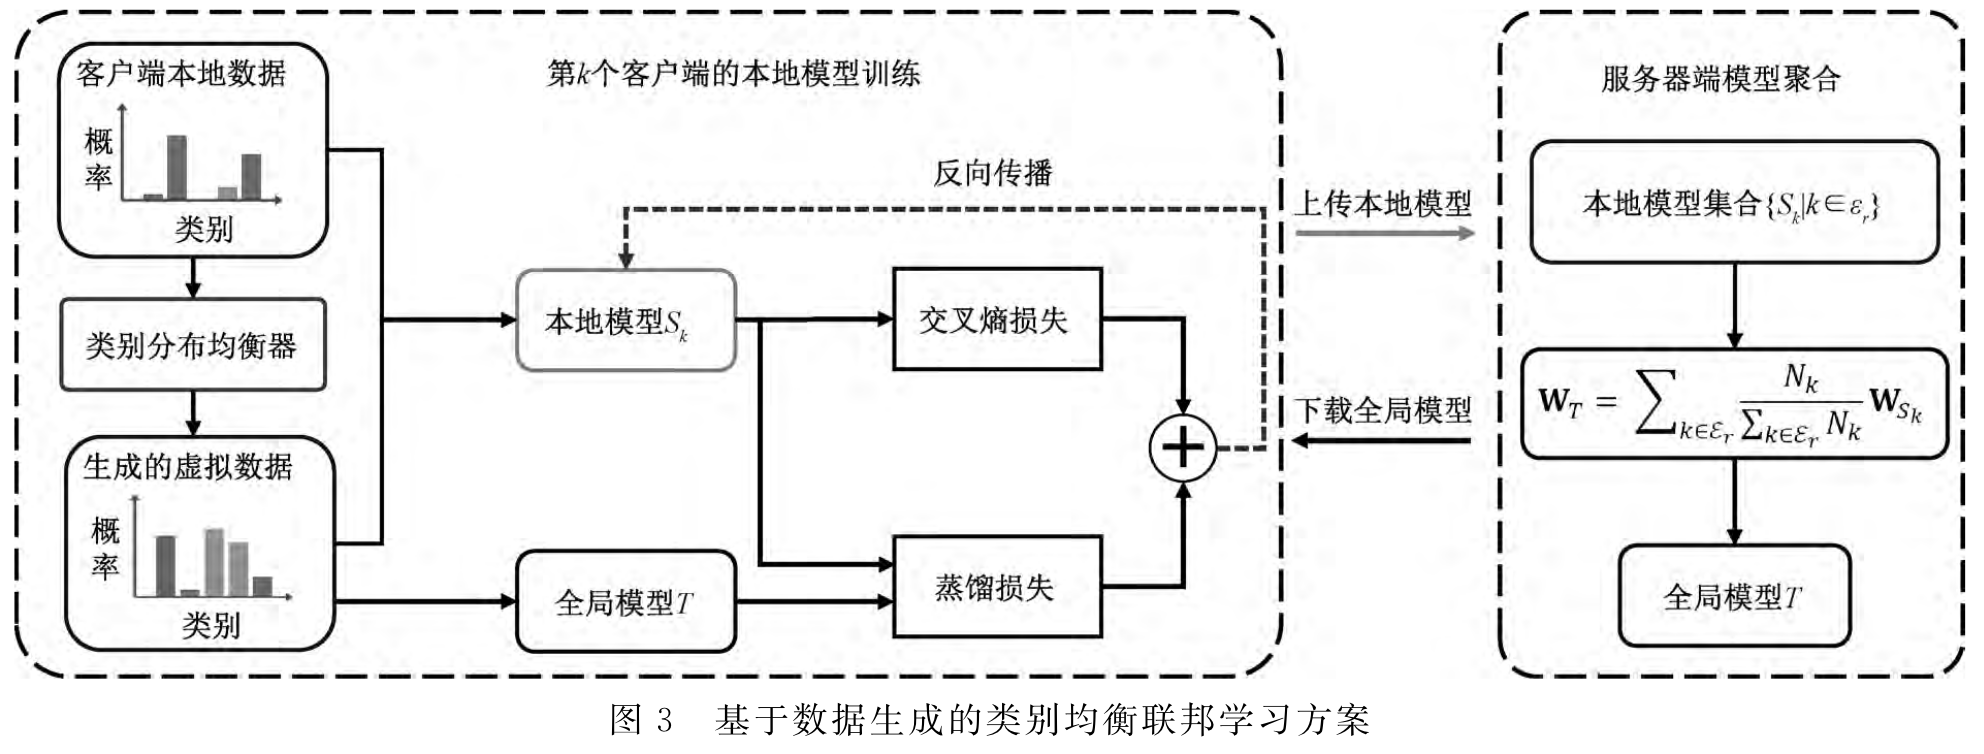
\includegraphics[width=1\textwidth]{images/img_overview}

\end{frame}

	


\begin{frame}{3.2 类别分布均衡器}{类别均衡采样器}


\begin{columns}
\begin{column}{0.5\textwidth}
\begin{figure}[ht]
\centering
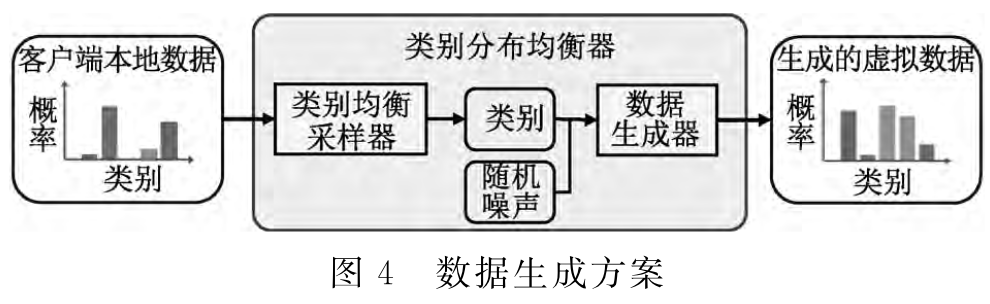
\includegraphics[width=1\textwidth]{images/img_gan}
\end{figure}

类别均衡采样器构造完成后, 各客户端根据采 样概率 $\widetilde{P}_m$ 采样相应的类别 $m$。 值得注意的是, 该过程在客户端进行, 客户端的数据分布信息不会发送至服务器端。
\end{column}
\begin{column}{0.5\textwidth}
(1) 统计客户端上类别 $m$ 的概率:
$$
P_m=\frac{n_m}{\sum_{m=0}^{M-1} n_m}
$$
(2)计算与客户端上类别分布相反的采样概率, 即类别 $m$ 的采样概率为:
$$
\bar{P}_m=1-P_m
$$
(3) 归一化采样概率:
$$
\widetilde{P}_m=\frac{\bar{P}_m}{\sum_{m=0}^{M-1} \bar{P}_m}
$$
\end{column}
\end{columns}


\end{frame}


\begin{frame}{3.2 类别分布均衡器}{数据生成器}
通过类别均衡采样器, 客户端可获得各类别的 采样量。 然而, 如何根据所采样的类别获得相应的 数据以用于本地模型的训练仍然是一个难题。 为解 决该问题, 本文引入了数据生成器 $G$。 该数据生成 器的输人为类别标签 $y$ 和噪声矢量 $z$。 其中 $y \in$ $\{0,1, \ldots, M-1\}, z$ 服从高斯分布 $N(0,1)$。 数据生 成器 $G$ 根据噪声矢量 $z$ 和类别标签 $y$ 生成相应的数据 $\hat{x}$, 即
$$
\hat{x}=G(z \mid y), z \sim N(0,1) 
$$
数据生成器和类别均衡采样器构造完成后, 客户端首先根据类别均衡采样器采样类别 $m$, 然后利用数据 生成器生成类别为 $m$ 的虚拟数据。 最后, 客户端结 合本地数据和生成的虚拟数据, 从而构造类别均衡 的数据集来训练本地模型。
\end{frame}


\begin{frame}{3.2 模型训练}{数据生成器的训练}
\begin{figure}[ht]
\centering
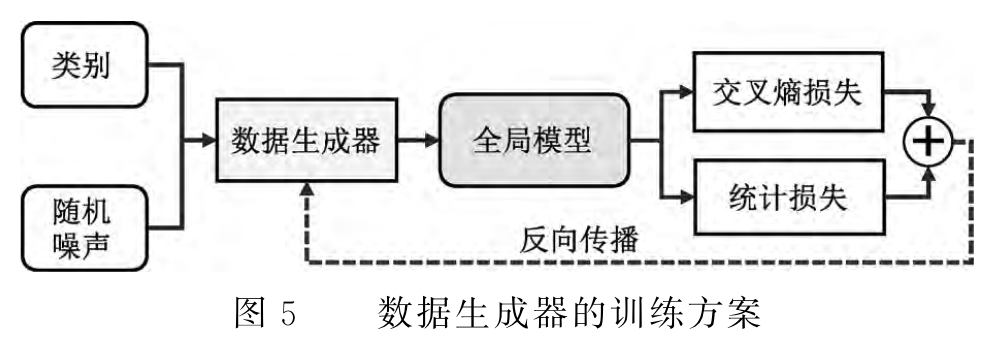
\includegraphics[width=0.8\textwidth]{images/img_gan_train}
\end{figure}
为训练数据生成器,一种常用的做法是采取对抗学习的方式。该方式需要额外训练一个判别器,且训练判别器需要相应类别大量的真实数据样本。本文提出利用全局模型的全局数据分布信息来训练生成器,从而无需训练判别器。
\end{frame}

\begin{frame}{3.2 模型训练}{本地模型的训练}


\begin{columns}
\begin{column}{0.5\textwidth}
\begin{figure}[ht]
\centering
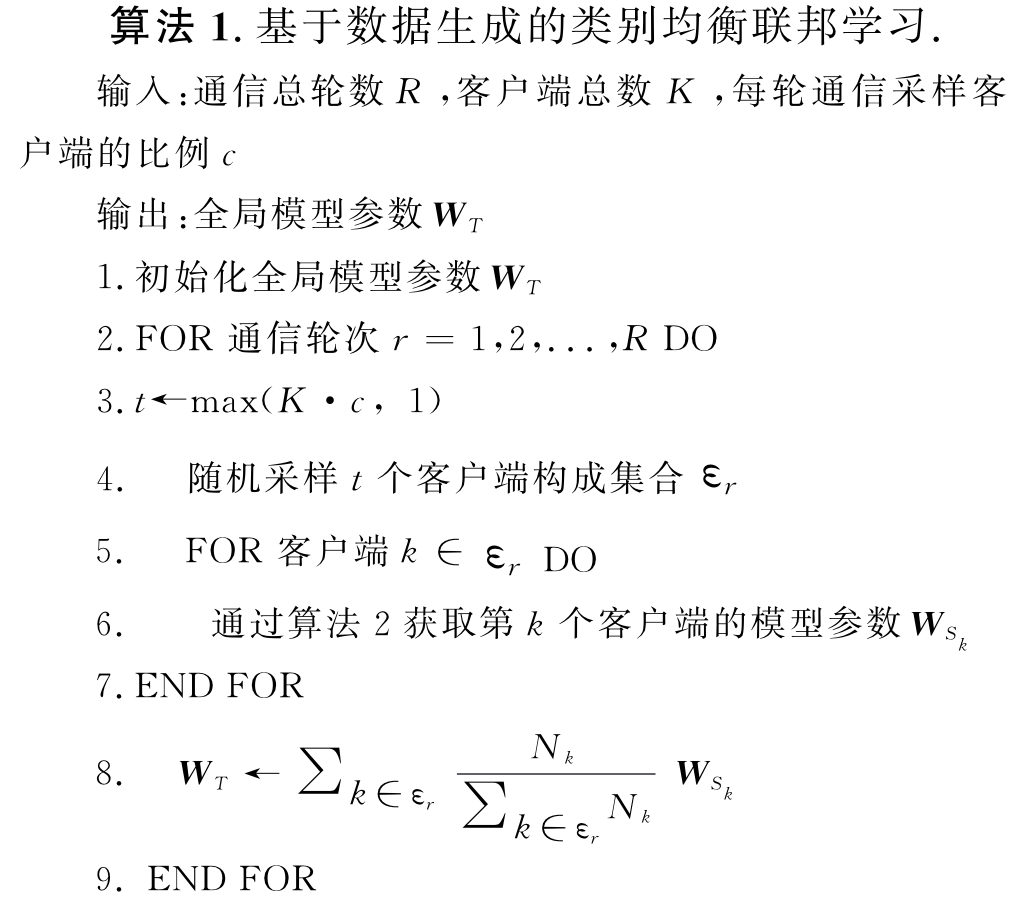
\includegraphics[width=1\textwidth]{images/algo1}
\end{figure}

\end{column}
\begin{column}{0.5\textwidth}
\begin{figure}[ht]
\centering
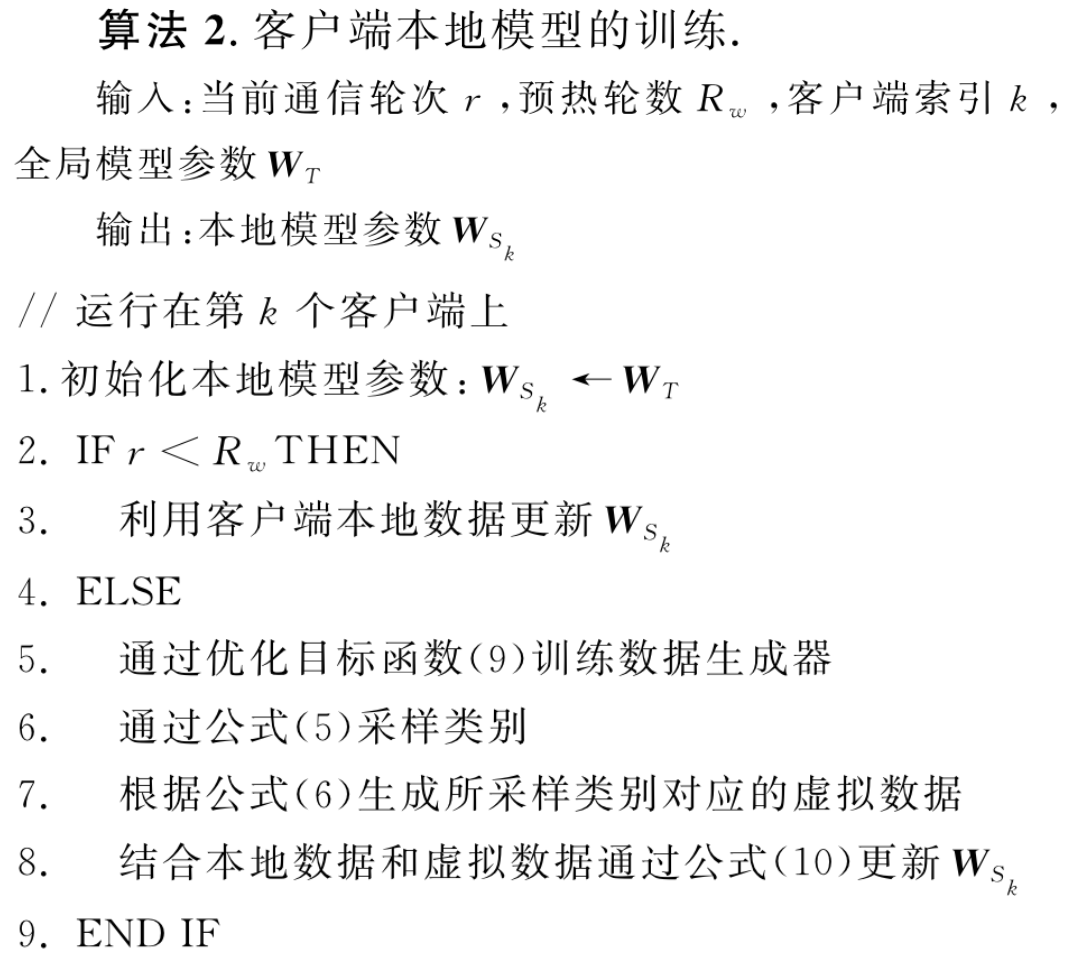
\includegraphics[width=1\textwidth]{images/algo2}
\end{figure}
\end{column}
\end{columns}


\end{frame}



\begin{frame}{3.2 模型聚合}
联邦学习通过聚合各客户端本地模型的参数获 得一个高性能全局模型。本文所提出的 CBFL 在客户端构造类别均衡的数据集来训练本地模型, 使得服务器端更易于聚合这些性能良好且差异性小的本地模型。参考 $\mathrm{FedAvg}, \mathrm{CBFL}$ 以 加权平均的方式聚合各本地模型的参数来更新全局 模型, 即
$$
\boldsymbol{W}_T=\mathbb{E}_k\left[\boldsymbol{W}_{S_k}\right]=\sum_{k \in \varepsilon_r} \frac{N_k}{\sum_{k \in \varepsilon_r} N_k} \boldsymbol{W}_{S_k} 
$$
通过上述公式, 全局模型汇聚各客户端本地模型的信息. 此外, 更新后的全局模型也将帮助数据 生成器获得更准确的全局数据分布信息.

\end{frame}




\section{实验分析}

\begin{frame}{4.1 数据集}

	\begin{itemize}
\item[1)] CIFAR-10由60000张32×32像素的彩色图像组成,共包含10个类别,每个类别包含6000张图像.训练集与测试集分别包含50000张和10000张图像; 
\item[2)] CIFAR-100与CIFAR-10的组成相似,但CIFAR-100包含了更多的类别.CIFAR-100共包含100个类别,每个类别包含500张训练图像和100张测试图像; 
\item[3)] CINIC-10包含270000张图像.值得一提的是,该数据集的图像不一定来自相同的分布.这个特性非常适合联邦学习,因为实际场景中各个客户端的数据不一定服从相同分布.CINIC-10具有相同大小的训练集、验证集和测试集.本文在训练集上进行模型训练,并在测试集上进行测试,而不使用该数据集的验证集; 
\item[4)] iNaturalist2019是一个大规模的类别分布高度不均衡的真实数据集.该数据集包含1010个类别,总计268243张彩色图片,由i Naturalist网站的2295个用户收集和上传.每个用户上传的图片被视为一个客户端的数据集.
\end{itemize}
\end{frame}

\begin{frame}{4.2 对比模型}
	本文将CBFL与目前最新的方法进行比较,即FedAvg、FedPoxr、SCAFFOLD和FedNvao.本实验通过狄利克雷分布Dir(0.1)模拟各客户端数据的类别分布.所有方法基于两种常见的深度神经网络模型(即ResNet20和MobileNet V2)进行训练和性能比较.
\end{frame}


\begin{frame}{4.3 实验结果}{Result Analysis}
	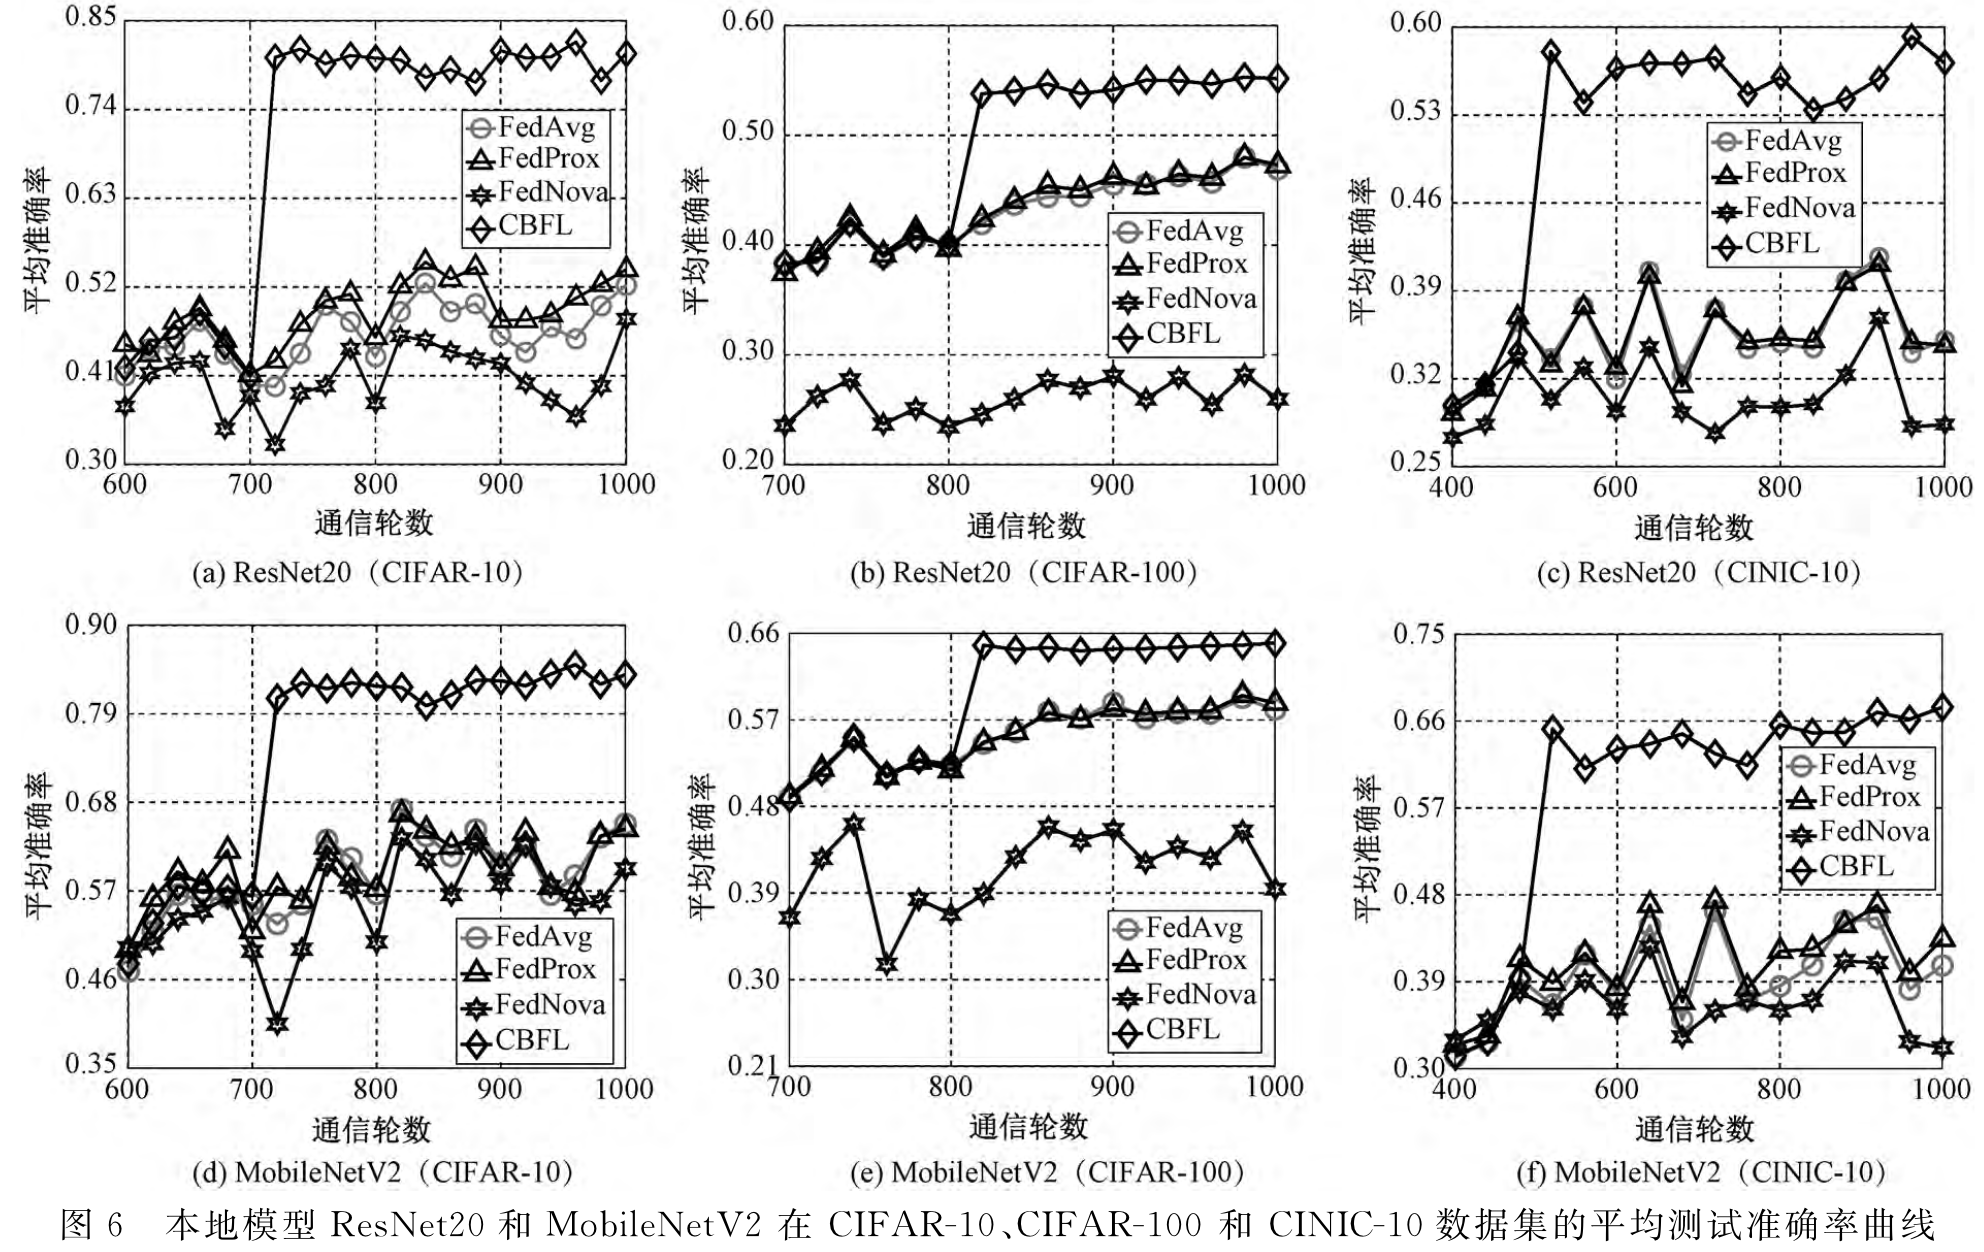
\includegraphics[width=0.75\textwidth]{images/img_expr1}
\end{frame}

\begin{frame}{4.3 实验结果}{Result Analysis}
	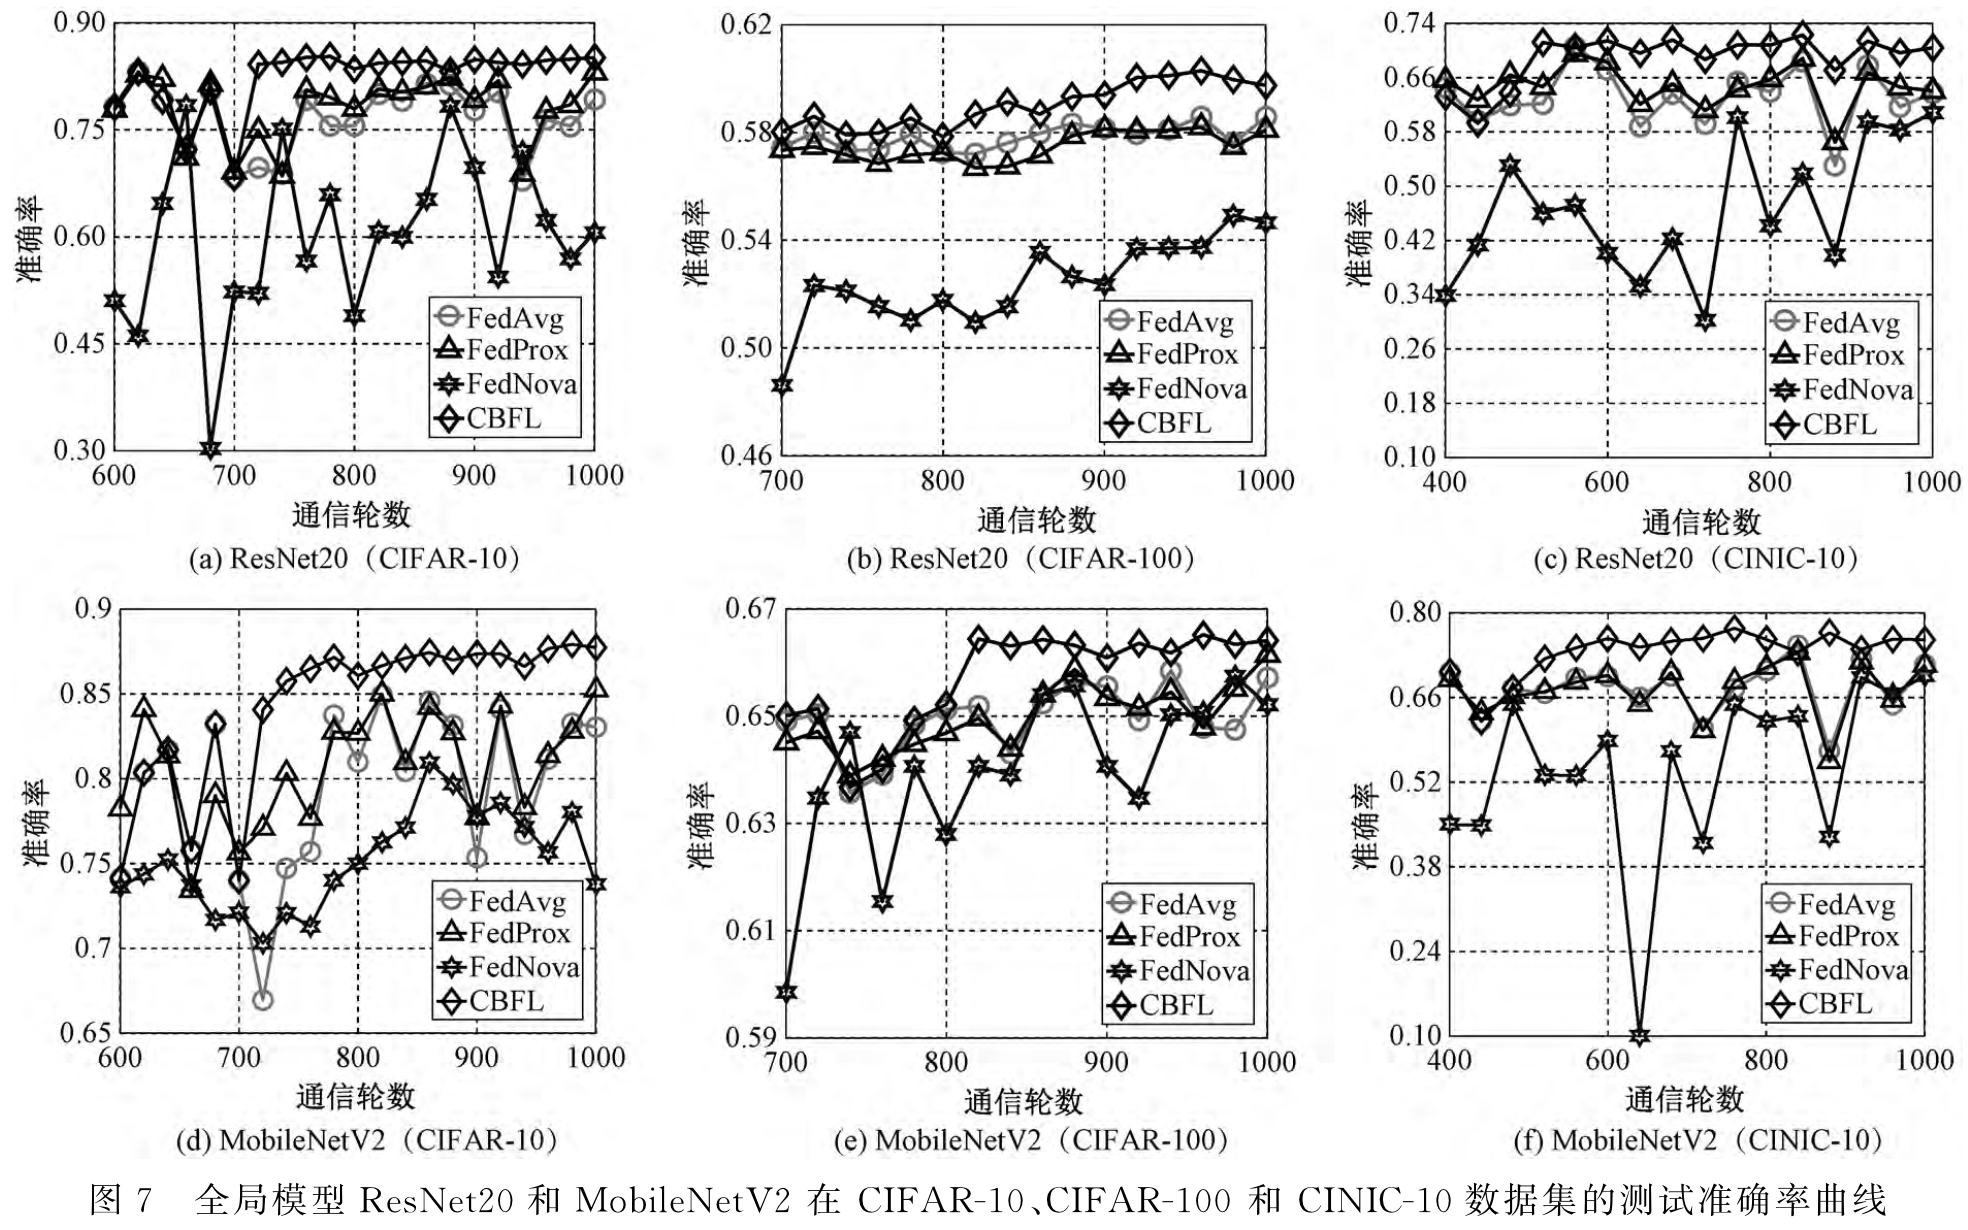
\includegraphics[width=0.75\textwidth]{images/img_expr3}
\end{frame}

\begin{frame}{4.3 实验结果}{Result Analysis}
	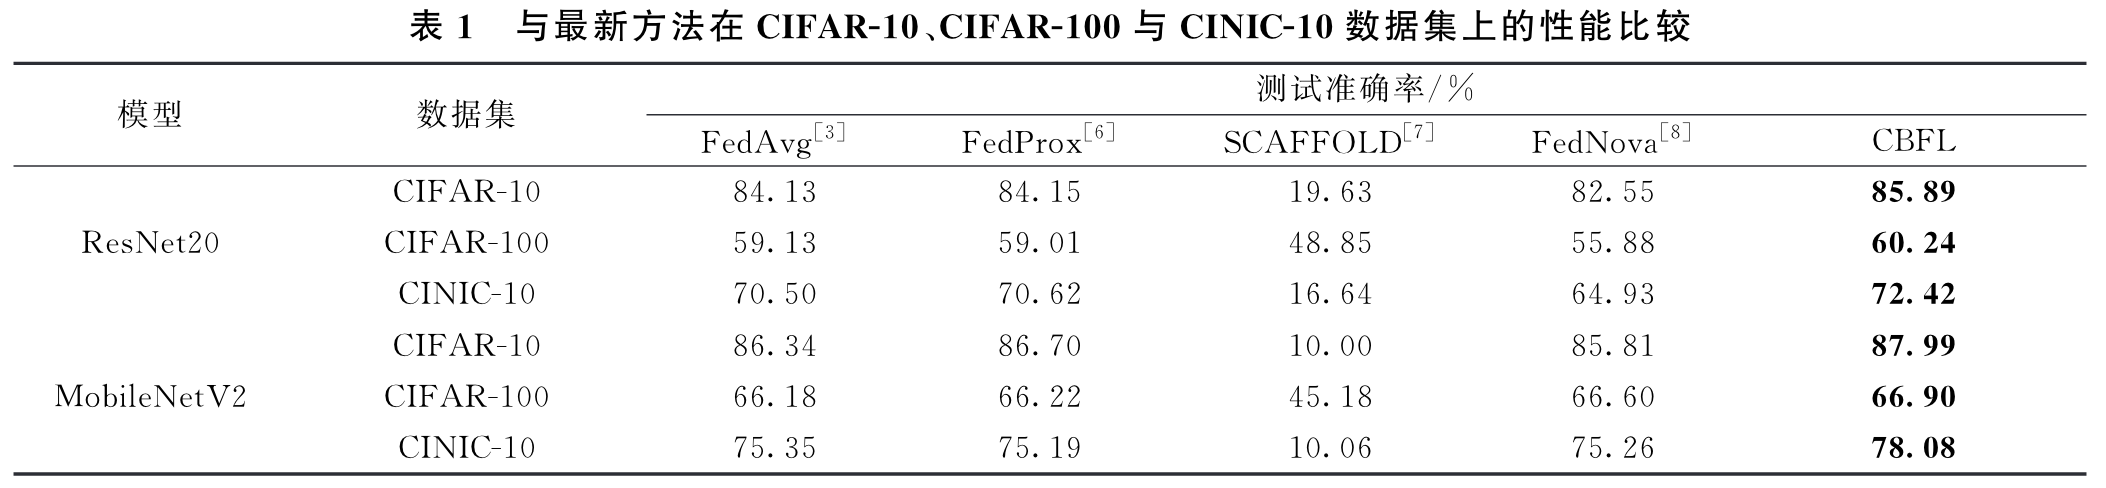
\includegraphics[width=1.\textwidth]{images/img_expr2}
\end{frame}

\begin{frame}{4.3 实验结果}{Result Analysis}
	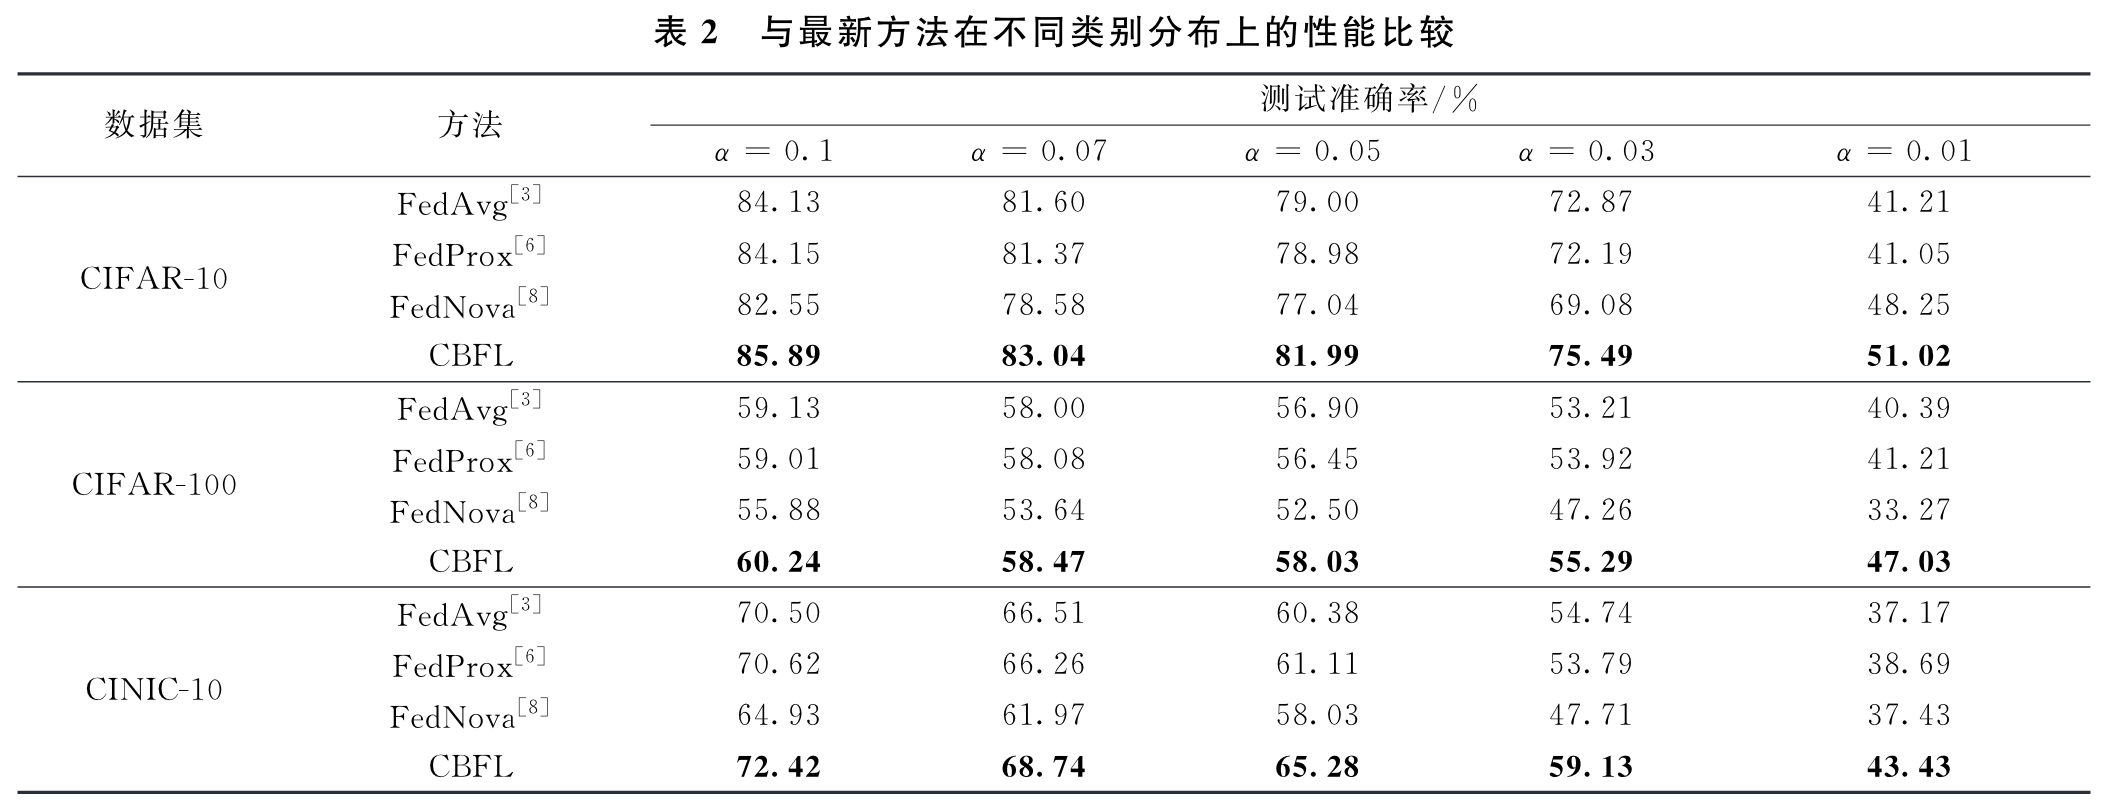
\includegraphics[width=1.\textwidth]{images/img_expr4}
\end{frame}



\section{研究总结}

\begin{frame}{研究总结}

本文提出了一种基于数据生成的类别均衡联邦学习(CBFL)方法.CBFL针对各客户端构造类别均衡的数据集,以降低客户端类别不均衡和客户端之间分布差异的影响.
\\ \hspace*{\fill} \\
具体而言,CBFL设计了一个类别分布均衡器,其由一个类别均衡采样器和一个数据生成器组成.其中,类别均衡采样器以较高概率采样客户端本地数据量不足的类别,然后,数据生成器根据所采样的类别生成相应的虚拟数据.结合本地数据和虚拟数据,客户端构造类别均衡的数据集来进行模型训练,从而有利于构建高性能全局模型.
\end{frame}



\backmatter

\end{document}
